\chapter{Available high-throughput normal human Datasets}
\label{ch:datasets}

\begin{comment}
\setlength{\epigraphwidth}{0.57\textwidth}
\setlength{\epigraphrule}{0.1pt}
\epigraph{Data! Data! Data! I can’t make bricks without clay!}{Sherlock Homes
    (Sir Arthur Conan Doyle)}
\end{comment}

In the past few years, many laboratories studied the expression
of the genes within normal humans at the transcriptome and at
the proteome levels. In this chapter, I review the data I use within my thesis
and how it has been processed.

When not stated otherwise, all the computational processing of the \Rnaseq\ part
described here have been performed by myself under the supervision of
the Dr Alvis Brazma. I also received general feedback from Dr Mar Gonzalez-Portà,
Dr Johan Rung and Dr Nuno Fonseca. The proteome data has been processed by
Dr James Wright from the Wellcome Trust Sanger Institute.


\section{Introduction}

Every dataset with which I worked is fitting three main criteria.
First, they comprise human normal samples from at least three kinds of tissues.
Secondly, they are non-targeted high-throughput \ie\ gene expression
quantifications are based on \Rnaseq\ for the transcriptome or on \ms\ for the
proteome. These technologies allow in theory to study the whole repertoire of
\glspl{RNA} or proteins in a sample.
Finally, the \emph{raw} data is available and reusable.

In the next section, I first describe the \Rnaseq\ and then the \ms\ data I use
in my thesis; then I detailed how these data have been processed before being
employed in the various analyses that compare the transcriptome and proteome
before attempting to integrate them together.


\section{RNA-Seq Transcriptome data}

There are a few more studies that I wanted to use on the
transcriptomic side, but the reusability point was often the critical reason
why they have not been included.

Indeed, many times I encountered data with ambiguous encoding format
and, as the studies were a little bit outdated,
I was also unable to get the information from the original authors.
I describe hereafter the 5 transcriptomic datasets I used
in the chronological order of their first public release.
\Cref{tab:Trans5DF} summarises the main characteristics of the different
datasets.

\begin{sidewaystable}
           \centering
           \caption{\label{tab:Trans5DF}General description of the 5 transcriptomic
           dataset (\Rnaseq) used for this study}
       \begin{tabular}{@{}cccccccccc@{}}
       \toprule
       \multicolumn{1}{c|}
           {\multirow{2}{*}{ArrayExpress ID}} &
            \multicolumn{1}{c|}{\multirow{2}{*}{Data ID}} &
            \multicolumn{2}{c|}{\begin{tabular}[c]{@{}c@{}}Library\\Preparation\end{tabular}} &
            \multicolumn{2}{c|}{Sequencing} &
            \multicolumn{2}{c|}{Replicates} &
            \multicolumn{1}{c|}{\multirow{2}{*}{\begin{tabular}[c]{@{}c@{}}Tissue\\
                    Number\end{tabular}}} &
            \multirow{2}{*}{\begin{tabular}[c]{@{}c@{}}Multi-sampling\\ from the \\ same
            individual\end{tabular}} \\
            \cmidrule(lr){3-8}
            \multicolumn{1}{c|}{} & \multicolumn{1}{c|}{} &
            \multicolumn{1}{c|}{\begin{tabular}[c]{@{}c@{}}Whole\\ RNA\end{tabular}} &
            \multicolumn{1}{c|}{\begin{tabular}[c]{@{}c@{}}PolyA\\ selected\end{tabular}} &
            \multicolumn{1}{c|}{\begin{tabular}[c]{@{}c@{}}Single\\ end\end{tabular}} &
            \multicolumn{1}{c|}{\begin{tabular}[c]{@{}c@{}}Paired\\ end\end{tabular}} &
            \multicolumn{1}{c|}{Biological} & \multicolumn{1}{c|}{Technical} &
            \multicolumn{1}{c|}{} &  \\
       \midrule
       E-MTAB-305 & Castle & Y &  & Y &  &  &  & 11 &  \\
       E-GEOD-30352 & Brawand &  & Y & Y &  & Y &  & 8 &  \\
       E-MTAB-513 & IBM &  & Y & Y & Y &  & (Y) & 16 &  \\
       E-MTAB-2836 \footnotesize{(and E-MTAB-1733)}& Uhlén &  & Y &  & Y & Y & Y & 32 &  \\
       E-MTAB-2919 & Gtex (v4)  & Y &  &  & Y & Y &  & 54 & Y \\
       \bottomrule
       \end{tabular}
\end{sidewaystable}

\subsection{Castle et al. dataset}

This dataset has been published along with the \paper{\citetitle{castleData}}
by \citet{castleData} who were interested in exploring the whole RNA repertoire
with sequencing-based technology. They essentially focused their study
on the non-coding part.

They used multiple-donors pooled tissues samples
and prepared the 11 libraries following a whole transcriptomic protocol
where nonribosomal \gls{RNA} transcripts are
specifically amplified by \gls{PCR} \citep{Armour:2009}.

They generated an average of 50 million sequence reads per tissue
using an Illumina Genome Analyser-II sequencer (single-end).
They trimmed their original reads to 28 \gls{nt}
and then released them through EMBL archives (\ENA{ERP000257}
and \ArrayExpress{E-MTAB-305}).

Despite several limitations (lack of replicates, old technology, small reads),
I used this dataset for two main reasons. First, it is the oldest available
\Rnaseq\ data I found that was performed on Human normal tissues. Thus, the
results congruence of this dataset to the others gives a rough assessment about
the extent of \Rnaseq\ datasets that can be integrated together in an atlas.
Secondly as \Rnaseq\ studies are prepared mainly with polyA-selected protocols
nowadays, I was interested to gauge how the library protocols --- and the
presence of \glspl{ncRNA} --- can affect the quantifications and then the final
outcomes.


\subsection{Brawand et al. dataset}

In the corresponding article entitled \paper{\citetitle{VTpaper}},
\citet{VTpaper} focused their interest on the
evolution of the mammalian transcriptomes --- while there were existing studies
on the matter, the sequencing approach was then creating new perspectives.

They collected 6 organs from 10 different vertebrates:
9 mammalians (including Human) and a bird. They have two biological replicates
per tissue: one male and one female for every tissue but the testis (two males).
They used a polyA-selected protocol to prepare their 131 libraries (including 23
for \species{Homo sapiens}).
Hence, the samples are largely enriched in protein coding genes.

They generated an average of 3.2 billion reads of 76 base pairs per sample
using an Illumina Genome Analyser IIx (single-end) and they released them
through \gls{GEO} (accession number: GSE30352).
I personally retrieved the human data from
\ArrayExpress{E-GEOD-30352}\footnote{ArrayExpress routinely imports
datasets from \gls{GEO} on a weekly basis.}.


\subsection{Illumina Body Map 2.0}
This dataset has been first created in 2010 and released in
2011\footnote{See: \citetitle{ibmEnsembl} - \cite{ibmEnsembl}} by Illumina
mostly to advertise its most recent technology improvement at that time:
the paired-end sequencing. Indeed, until then, all the sequencing was done
from only one end of the \gls{DNA} or \gls{cDNA} fragments.\footnote{From that
date, most of the following transcriptome studies based on \Rnaseq\ are using
paired-end sequencing.}

It comprises 16 tissues (one donor per tissue), which were prepared with a
polyA-selected library preparation protocol.

Although each sample has been sequenced twice and that we have in principle
\emph{technical} replicates, these are not ``regular'' technical
replicates. \emph{Technical} replicates,
by contrast to \emph{biological} replicates,
usually imply that their processing uses the same sample source and protocols.
Thus, the error and the noise due to a specific technique could be determined.
Here, however, each tissue has been sequenced once with a singled-end protocol
and once with a paired-end one.

The sequencing was performed with an Illumina HiSeq 2000 and the reads were
released through \ArrayExpress{E-MTAB-503} (\ENA{ERP000546}), from where I
retrieved the single-end and paired-end mono-tissue samples.

Despite the lack of biological replicates, I used this dataset as it was for an
extended time the most extensive freely available \Rnaseq\ dataset of human
tissues and such has been referenced many times since it was released.

\subsection{Uhlén et al. dataset}

Uhlén et al.\ have created an atlas,
\href{http://www.proteinatlas.org/}{Human Protein Atlas}\footnote{%
Human Protein Atlas ---
\href{http://www.proteinatlas.org/}{http://www.proteinatlas.org/}},
revolving mostly around the spatial
distribution of the proteins through the Human body. They use many approaches
and techniques which also include \Rnaseq. They first released their \Rnaseq\
data of 27 normal tissues as a part of their article \paper{\citetitle{Uhlen2014}}
\citep{Uhlen2014}. Later, they extended their dataset with new samples and 5 new
tissues. The latest version was published with \paper{\citetitle{Uhlen2015}}
\citep{Uhlen2015} in \textit{Science}.

They provide (at least two) \emph{biological} replicates for the 32 tissues.
Except for a very small number, the tissues have both male and female donors.
There are also many \emph{technical} replicates.

The 200 libraries have been prepared following a polyA-selected protocol and
have been sequenced (paired-end) with an Illumina HiSeq 2000 or 2500. I started
to work with the first version (\ArrayExpress{E-MTAB-1733}) and then
with the extended version (\ArrayExpress{E-MTAB-2836}).

At the time of the redaction of this thesis, this dataset is the freely available
most important one either regarding the number of tissues
(see \Cref{tab:Trans5DF}) or the number of samples (see \Cref{tab:Lib5DF}).


\subsection{GTEx data}

The Genotype-Tissue Expression (\gls{GTEx}) project is funded by the \gls{NIH}
Common Fund and aims to establish a resource database and associated tissue bank
for the study of the relationship between genetic variation and gene expression
and other molecular phenotypes in multiple reference tissues. The project was first
explained in a paper from the \cite{GTEx2013}. It consists to quickly collect
many tissues from postmortem donors so genotype-tissue expression analyses could
be done, notably \gls{eQTL} variants studies which study the modulation
of \gls{RNA} expression in function of \glspl{SNP}. The results of the
analyses are released through the GTEx portal\footnote{\Gtex\ portal --- %
\href{http://gtexportal.org}{http://gtexportal.org}}.

As the project is quite ambitious and the collection and sequencing of the samples
are taking time, several freezes of the data have been released. My work is
including samples up to the fourth release of the pilot phase (v4). This
release includes 54 tissue/cell types (53 normal and 1 tumour)
collected on 551 individuals.
The 3,276 libraries were prepared from whole \gls{RNA} extracts and then sequenced
with a paired-end protocol on Illumina HiSeq 2000/2500 sequencers which produced
an average of 80 million reads.

For privacy reasons, the raw data is available only through controlled access via
\dbGaP{phs000424.v4.p1} (access number specific to the version of the data I used
in my study). While getting access can take time, in principle every request for
academic research should be granted.

\section{Mass spectrometry Proteome data}

While the transcriptomic data was retrieved and then processed within the \EBI\
either by Dr Nuno Fonseca or myself, the proteomic data have been picked and
handled by Dr Jyoti Choudary and Dr James Wright from the Wellcome Trust
Sanger Institute.

Until a couple of years ago, compared to the transcriptome, the proteome world
was regrettably lacking on normal human tissues expression quantification
experiments. In fact, while there were human protein maps available
(\eg\ the \href{www.proteinatlas}{Human Protein Atlas}%
\footnote{Human Protein Atlas --- \href{http://www.proteinatlas.org}%
{www.proteinatlas.org}}), these
are mostly reporting the spatial expression of proteins (as they are based
on immunohistochemistry or other means of identification) than quantifying
their (non-targeted) abundance in each tissue.

Then, in 2014, two different groups of authors, \cite{PandeyData}
and \cite{KusterData}, published (in \textit{Nature},
issue 7502) their own \emph{``draft of the human proteome''}
based on the study of tissues with \ms. These two datasets complement a previous
smaller one that was publicly released but never published.

Hereafter, I present these 3 datasets that I use in my thesis.

\subsection{Pandey Lab data}

The Pandey Lab \citep{PandeyData} created the
\href{http://www.humanproteomemap.org/}%
{Human Proteome Map}\footnote{Human Proteome Map --- %
\href{http://www.humanproteomemap.org/}{www.humanproteomemap.org}} which
they released along \paper{\citetitle{PandeyData}}.

For their study, they have processed 30 kinds of histological normal human
tissues and cell line samples (17 adult tissues, 7 fetal tissues and 6
haematopoietic cell types). The samples were created from pooled samples of three
individuals (generally two males and one female).

Then, they prepared their libraries with a label-free method to quantify
as many proteins they could. They fractionated the samples to protein level by
\gls{SDS-PAGE} and then at peptide level by \gls{RPLC} to create 85 experimental
samples. Finally, they use state-of-art \gls{MS/MS} protocols
(with high-resolution and high accuracy \glspl{FTMS}:
Thermo Scientific Orbitrap instruments).
They generated about 25 million of (\gls{HCD})
high-resolution mass spectra which account for 2,212 \gls{LC-MS/MS} profiles.

The raw spectra were retrieved from ProteomeXchange via the repository
\Pride{PXD000561}.

While their effort to generate high quality raw data was highly appraised
by the scientific community, their processing
(identification and quantification) methods were
criticised (see~\cite{Ezkurdia2014-qx}). Thus, for this thesis I only use
quantification that James Wright provided me after reprocessing the dataset
from the raw spectra.

\subsection{Kuster data}

As for the Kuster Lab approach of the human proteome map,
\cite{KusterData} combined newly generated \gls{LC-MS/MS} spectrum
data (about 40\%) with already published one
(either from their colleagues or accessible through repositories ---
for the remaining 60\%).
The data comprised 16,857 experiments involving tissues, body fluids and cell
lines. They used all the data they could access from \gls{PTM} to affinity
purification studies.

They reprocessed the whole collection of spectra to maximise proteome coverage
and make it available through their own repositories: ProteomicsDB\footnote{%
Proteomicsdb --- %
\href{https://www.proteomicsdb.org/}{www.proteomicsdb.org}}.

The subset of data considered in my thesis is also
known as the [protein] Human BodyMap which is the part that was primary generated
by the Kuster lab itself for this study. It corresponds to 1,087 \gls{LC-MS/MS}
profiles and comprises 48 experiments covering 36 tissues (adult and fetal) and
cell lines. Overall that represents about 14 million of (\gls{HCD}/\gls{CID})
spectra from Thermo Scientific instruments.

This raw data was downloaded from \Proteomicsdb{PRDB000042}.

\subsection{Cutler data}
\begin{comment}
    rexpliquer quelle partie reutilisée
\end{comment}

This data was generated prior to the \dataset{Pandey} and the \dataset{Kuster}
data as it was released in 2011 through PeptideAtlas\footnote{PeptideAtlas --- %
\href{http://www.peptideatlas.org/}{www.peptideatlas.org}}
\citep{PeptideAtlas}.

It was created by Paul Cutler at Roche Pharmaceuticals.
It comprises 10 different tissues (1,618 \gls{CID} Thermo Scientific raw files).

While this data was never published on its own, it has been used in different
studies. Indeed, the \dataset{Cutler} data is one the datasets that
\cite{KusterData} are using in their original study to create ProteomicsDB.

The raw files were accessed and downloaded from \Proteomicsdb{PRDB000012}.

\section{Constant processing pipelines}

For many reasons, I only used data reprocessed from raw files despite many
ready available quantifications for most of the datasets.

In fact, original authors often released themselves their quantification values
either directly (\eg\ \cite{Krupp2012})
or only upon requests (\eg\ \cite{PandeyData}). Unfortunately, each study has
been processed with a different protocol, \eg\ \dataset{\Gtex}
data \citep{GTExTranscript} and \dataset{Castle} data \citep{Krupp2012}.

Third-parties could also distribute quantification of expression values either
retrieved from the original studies, as BioGPS \citep{BioGPS1} or
Harmonizome \citep{Harmonizome}, or achieved after reprocessing the raw data
as EBI Gene Expression Atlas \citep{EBIgxa} does.

Alas, from the time I started my study till the redaction of the current thesis,
the available quantifications were still products of different methodologies%
\footnote{Nowadays, I would though be able to use
quantification data directly downloaded from \EBI\ Gene Expression Atlas for
most of the analyses of this thesis.}.

Intuitively, we expect that different processing protocols produce
different results.

Indeed, along my work, I noticed many potential bias sources that impact
\Rnaseq\ outputs. Many of them have since then been reported in the literature;
annotations \citep{annotationDiff},
contamination \citep{contaminationRNAseq},
quality controls \citep{qualityRNAseq} and
mapping and quantifications pipelines \citep{Fonseca2014}
have great effects on the final quantification. Lastly, normalisation
methods also greatly impact the final expression values
\citep{Dillies2013}, \citep{normalisation2}.

For all these reasons, reprocessing all the transcriptomic datasets was the
logical first step of this current study.

Likewise, the proteomic datasets were uniformly reprocessed from the raw spectra
by Dr James Wright. In fact, there are various methods and several parameters
to pick for each of the many processing steps needed between the peptide
identification and the normalisation of the protein expression values.


\subsection{Transcriptome RNA-Seq raw data processing}

While I downloaded and entirely processed four of the transcriptomic datasets
myself (\dataset{Castle}, \dataset{Brawand}, \dataset{IBM} and \dataset{Uhlén}
data), it was not the case for the \Gtex\ dataset.

Since the \Gtex\ data is involved in many project within the \EBI\
and due to its huge amount of files (number and  size -- see \Cref{tab:Lib5DF}),
it was agreed that this would be processed centrally by one person and then
redistributed to all the other interested parties. Dr Nuno Fonseca had this
tremendous task and provided me with quantification data (produced with the
Human genome GRCh38 and ENSEMBL 76 annotation).

\begin{table}
\centering
\caption[Technical description of the 5 transcriptomic datasets]{%
\label{tab:Lib5DF}\textbf{Technical description of the 5 transcriptomic
    datasets}\\\footnotesize{I processed all the datasets but the one in
    \textit{\color{darkgray}italic}.\\
    For the Brawand dataset, I only processed the \species{Homo sapiens} part.}}
\begin{tabular}{@{}cccccc@{}}
\toprule
Dataset & \begin{tabular}[c]{@{}c@{}}Sample number\\(biologic)\end{tabular} &
\begin{tabular}[c]{@{}c@{}}Library\\number\end{tabular} &
\begin{tabular}[c]{@{}c@{}}File\\number\end{tabular} &
\begin{tabular}[c]{@{}c@{}}Total size of\\the fastq\\raw files (GB) \end{tabular}&
    \begin{tabular}[c]{@{}c@{}}Mean number of\\biologic samples per\\tissues
    [min,max]\end{tabular} \\
\midrule
Castle        & 11    & 11    & 11    & 58    & 10 (mixture)    \\
Brawand       & 18    & 21    & 23    & 111   & 2.8  [2,3]      \\
{\small Illumina Body Map} & 16    & 36    & 48    & 1,004  & 1 \\
Uhlén         & 122   & 200   & 400   & 1,851  & 3.81    [2,11] \\
    \textit{\color{darkgray}\Gtex\ (v4)}  &
    \textit{\color{darkgray}3,276}  & \textit{\color{darkgray}3,276}  &
    \textit{\color{darkgray}6,552}  &
    \textit{\color{darkgray}$\sim$ 50,000}  & \textit{\color{darkgray}60.67 [4,214]}\\
\bottomrule
\end{tabular}
\end{table}

For the sake of consistency and to avoid more biases \citep{h38vsh37},
that led me to reprocess all the other four \Rnaseq\ datasets
to comply with the reference used for the \Gtex\ samples. Actually,
as I accessed the datasets through an extended period of time, for a subset of
the datasets, I produced many sets of results with the previous human reference
genome (GRCh37) and three different ENSEMBL annotations (73, 74 and 75). The
results are congruent together hence supporting the robustness of the findings
presented in this thesis.

Hence, unless indicated otherwise, the results presented in the current work are
from these genome reference and annotation version.

In the early stages of my research, I was processing each of the different steps
sequentially and semi-manually with the help of custom made scripts.
While the \EBI\ cluster greatly facilitated the handling of the numerous files,
the task was quite tedious: particularly due to the necessary jobs monitoring of
each step and the integrity checks of the intermediate files between them.
Additionally, although working perfectly within the \EBI\ infrastructure,
the scripts I wrote would need a fair amount of work to achieve reproducibility
with another platform.

Fortunately, Dr Nuno Fonseca developed and released
an ``integrated RNA-seq analysis Pipeline'': \irap\footnote{\irap\ ---
see: \href{https://nunofonseca.github.io/irap/}%
{https://nunofonseca.github.io/irap/}}.
This tool allows the automation of the typical
(and state-of-the art) workflow to study
\Rnaseq. Apart of remarkably speeding up the data processing, it also
decreases the risk of inconstant parameters from one script to another.

\irap\ takes as input raw transcriptomic files encoded as \emph{\fastq}
files and a configuration file which precisely describes the dataset ---
its design (\eg\ groups of biological or
technical replicates) and technical (\eg\ encoding format, read length, paired-end or
single-end, \ldots) normalisation method to apply to the
quantification, \ldots) ---
and the tools, reference and annotations that should be used.
\begin{comment}
While the
configuration is exhaustive and takes time to be written, it is then really easy
to try out different set of parameters.
\end{comment}

Hence, all the transcriptomic datasets (either the ones I processed or \Gtex\
which was processed by Dr Nuno Fonseca) have been processed in their final
version with the same pipeline involving the same order of steps and the same
set of tools and versions.


\subsubsection{Data retrieval and preparation}

The human raw data of each dataset were retrieved from \gls{ArrayExpress},
\gls{ENA} and, once the access was approved, from \gls{dbGaP}.
Files encoded in a non-compliant format to the most recent tools (\dataset{Castle}
dataset) were translated to \gls{Phred} $33$ \fastq\ files with the help of
a \emph{perl} script (see~\Cref{code:fastq}).


\subsubsection{Data processing with iRAP}

\irap\ accepts as input these \fastq\ (or \gls{BAM}) files and manages all
the steps from the quality assessments till the quantification (and
normalisation) of the data.



Then, reads that present an overall quality score below a given threshold (10) are
fully discarded. Reads that have uncalled bases (\textsc{N}) are also discarded.
Since the quality decreases as the calling process progresses, all the reads are
trimmed to a same length\footnote{This is a requirement of some tools (mappers
in particular).} in a way to optimise the purity-length balance. The trimming has
to be less than 15\% of the original length. If needed, more reads are discarded
so the length is maximised.

Reads that could be assigned to a likely contamination source (here
\species{Escherichia coli}) are also discarded. This requires a first mapping
step to all the possible contaminant genomes. Reads that map to these genome
without ambiguity are discarded.

Finally, if the sequencing protocol is paired-end, all the ``orphan'' reads are
gathered together in a separate file as a subset of tools mishandle unmatched
paired-end reads.

These assessments and trimming have been performed with \soft{FASTX}
toolkit\footnote{\soft{FASTX} toolkit ---
\href{http://hannonlab.cshl.edu/fastx\_toolkit/}%
{http://hannonlab.cshl.edu/fastx\_toolkit/}} (0.0.13).

The mapping to contaminant genomes is done with a splice non-aware mapper:
\soft{BWA}\footnote{\soft{BWA} --- \href{http://bio-bwa.sourceforge.net/}%
{http://bio-bwa.sourceforge.net/}} (0.7.4).

\subsubsection{Mapping}
I chose to map the reads to the \species{Homo sapiens} genome with a spliced
read mapper: \soft{TopHat}\footnote{\soft{TopHat} ---
\href{https://ccb.jhu.edu/software/tophat/index.shtml}%
{https://ccb.jhu.edu/software/tophat/index.shtml}} (2.0.12) with the default
parameters.

While in the earlier stages of my work, I was using the GRCh37.p12
(GENCODE release 18) and then GRCh37.p13 genebuild (GENCODE release 19),
the complete set of datasets has been processed with GRCh38.p1.
When not stated otherwise, the presented results are from the GRCh38.p1 build.

\subsubsection{Quantification}
Two tools have been used for this step: \soft{HTSeq-count}\footnote{%
\soft{HTSeq-count} --- \href{http://www-huber.embl.de/HTSeq/doc/index.html\#}%
{http://www-huber.embl.de/HTSeq/doc/index.html\#}}(0.6.1p1) (intersection
non-empty mode) and \soft{Cufflinks}\footnote{\soft{Cufflinks} ---
\href{http://cole-trapnell-lab.github.io/cufflinks/manual/}%
{http://cole-trapnell-lab.github.io/cufflinks/manual/}} (2.2.1).

I am using only gene levels quantification and not isoforms.

\subsubsection{Normalisation}
\gls{RPKM}
values were then calculated with the internal function provided by \irap. For each
tissue, gene expression levels were calculated by first taking the mean of the
technical replicates before calculating the mean of the biological ones. When the
VEGA IDs of the genes had corresponding ENSEMBL 76 gene IDs, those IDs were
directly used to assess the gene expression. When this was not the case, the
coordinates of the genes were retrieved from the latest VEGA release and then the
windows of interest were plotted on merged bam files (one bam per tissue)
obtained from TopHat2. The Supplementary Dataset 1 includes the number of
paired reads that have been counted for each novel gene on the merged bam files
normalized by the number of initial samples for each tissue.



\subsubsection{Tissue Averaging}
Average Number of samples per tissues different => quantification averaged for
most of the analysis to avoid skewness.





\begin{figure}
    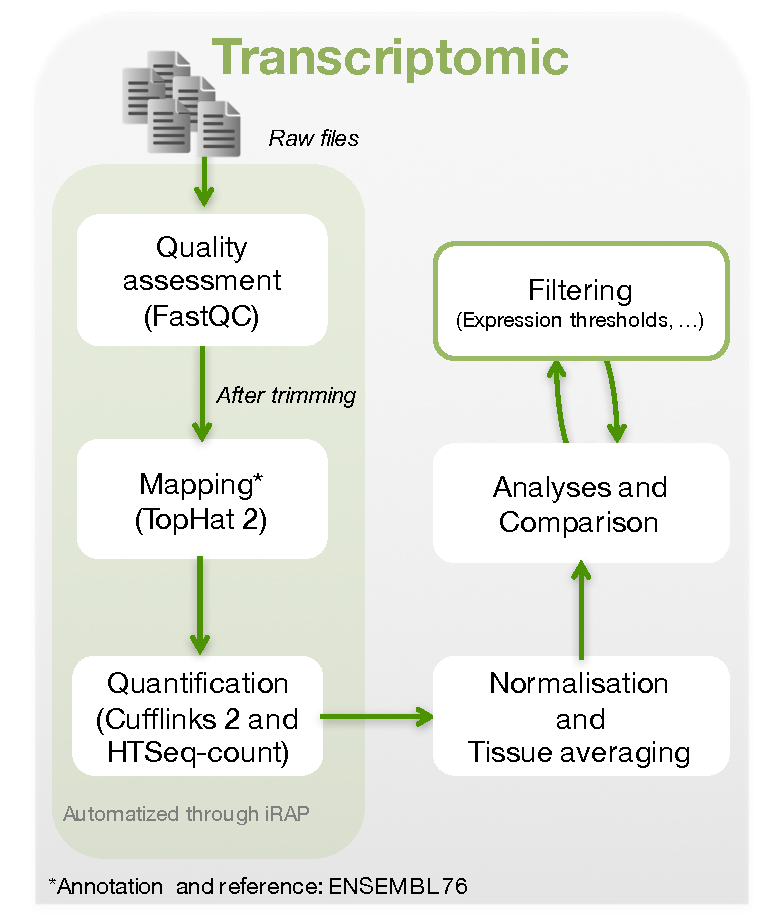
\includegraphics[scale=0.75]{additional/pipelineTrans.pdf}\centering
    \caption[General steps for processing the transcriptomic
    data]{\label{fig:pipelineTrans}\textbf{General steps for processing the
    transcriptome} [TK]}
  \end{figure}


\subsection{Proteome raw data}

Similarly to the transcriptome issue, there is the proteome which is actually
trickier (possible problem with Pandey data analyses). Really depends which
threshold and \gls{FDR} tolerate. And what database and algorithm are used to perform
the identification of the proteins. More messy.

All the data has been processed by James.

Small problem about mapping back proteins to transcripts.



And again describe the methodology.

  \begin{figure}
      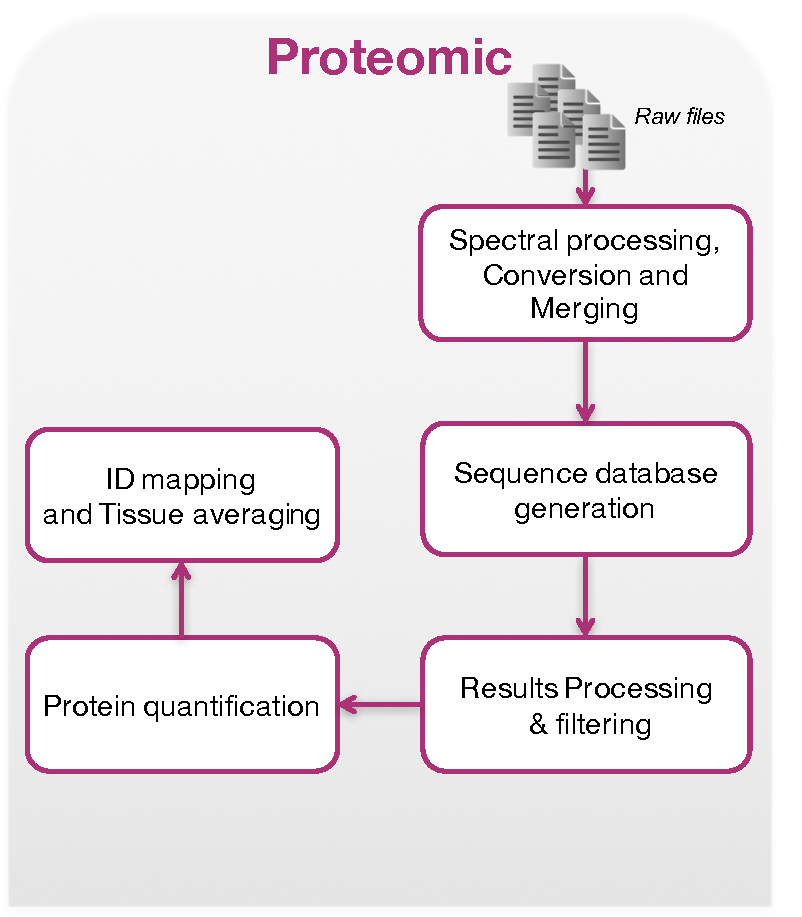
\includegraphics[scale=0.75]{additional/pipelineProteins.pdf}\centering
      \caption[General steps for processing the proteome
      data]{\label{fig:pipelineProt}\textbf{General steps for processing the
      proteome} [TK] }
  \end{figure}

\section{Discussion/Conclusion}

In this chapter, I describe why and how 5 transcriptomic and 3 proteomic normal
human tissues datasets have been reprocessed from raw files with unified
pipelines using the same reference and annotation files.




\TK{
Many tools are for now not a better than the other one. Can be hard to decide
which one to pick. A lot of decision have to been taken --- and while this
doesn't affect the overall landscape, if one is interested by a specific
genes, \Rnaseq\ should be supported with more wet-lab thing.\\
    Add shortly other important information (or maybe mix in a bit of discussion.
Too vague now) to the conclusion \\
All but one of these datasets have been subject of one if not more papers:
results confirmed previous authors.\\
Similar expression between HTSeq and Cufflinks
\\
Add the end of the day, \Rnaseq remains an exploratory (even when we look at
specific differential expression) studies.
}
